%%%%%%%%%%%%%%%%%%%%%%%%%%%%%%%%%%%%%%%%%%%%%%%%%%%%
%%%% En-tête leçon
\begin{headerBlock}
  \chapter{Phénomènes de résonance dans différents domaines de la physique}
  \label{LP_resonance} 
\end{headerBlock}




%%%%%%%%%%%%%%%%%%%%%%%%%%%%%%%%%%%%%%%%%%%%%%%%%%%%
%%%% Références
\begin{center}
\begin{tabularx}{\textwidth}{| X | X | c | c |}
  \hline
  \rowcolor{gray!20}\multicolumn{4}{c}{Bibliographie de la leçon : } \\
  \hline 
  Titre & Auteurs & Editeur (année) & ISBN \\
  \hline
  & & & \\
  \hline 
  & & &    \\
  \hline 
  & & &    \\
  \hline 
\end{tabularx}
\end{center}

%%%%%%%%%%%%%%%%%%%%%%%%%%%%%%%%%%%%%%%%%%%%%%%%%%%%

%%%%%%%%%%%%%%%%%%%%%%%%%%%%%%%%%%%%%%%%%%%%%%%%%%%%
%%%% Plan
\begin{reportBlock}{Plan détaillé}

  \textbf{Niveau choisi pour la leçon :} Licence 3
  \newline
  \textbf{Prérequis} : \begin{itemize}
      \item Mécanique newtonienne
      \item Optique ondulatoire
      \item 
  \end{itemize}

  \textbf{Déroulé détaillé de la leçon: }  
  
  \section*{Introduction}
Définition : pour un système auquel qu'on soumet à une excitation sinusoïdale de pulsation $\omega$, la réponse du système est maximale à la pulsation $\omega_0$, appelée fréquence de résonance.
  \section{Oscillateurs harmoniques amortis}
  \subsection{Résonance en vitesse en régime forcé} 
\textcolor{red}{Attention, faire la discussion sur la phase}. Interprétation énergétique possible.
  \section{Oscillateurs couplés}
\begin{center}
    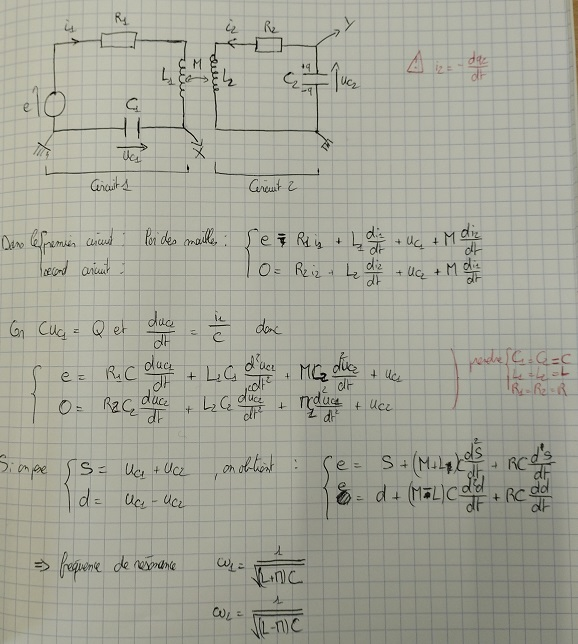
\includegraphics[scale=0.5]{LP_Resonance/Oscillateurs_couple.jpg}
\end{center}    


\textcolor{blue}{Expérience : }montrer l'influence du couplage sur la résonance du premier circuit RLC à l'aide d'un deuxième circuit RLC. Intérêt pratique ?

\section{Cavité résonante}
\end{reportBlock}